\begin{problem}{레이저 연구소}{표준 입력(stdin)}{표준 출력(stdout)}{2\,초}{1024\,MB}
    
아무도 모르는 외딴 섬에서 ahgus89와 Sait2000은 레이저 연구를 하고 있다. 이 섬에는 다양한 연구 구역이 있고, 그 중 레이저 연구 구역은 $N \times M$ 모양의 직사각형 영역이다. 이 영역은 $NM$개의 $1 \times  1$ 정사각형으로 쪼개져 있다. 각 정사각형의 꼭짓점에는 건물이 하나씩 세워져 있으며, 각 정사각형의 변에는 건물을 잇는 벽이 하나씩 세워져 있다. 따라서 총 $\left(N+1\right)\left(M+1\right)$개의 건물과 $2NM+N+M$개의 벽이 있다.

ahgus89와 Sait2000은 레이저의 성능을 시험하기 위해 건물에서 건물로 레이저를 쏘아 보려고 한다. 이들은 가능한 모든 시작점과 끝점에 대해 레이저를 쏠 것이다. 하지만 레이저는 직선으로만 나가기 때문에 건물과 벽이 레이저를 가로막을 수 있다. 

ahgus89는 출력을 강하게 하여 건물과 벽에 구멍을 내어서라도 실험을 하려고 한다. 시작점과 끝점에 있는 건물을 포함하여, 경로 상에 있는 모든 건물과 벽에 구멍이 뚫린다. 레이저가 정확히 건물을 통과할 경우, 그 건물에 붙어 있는 벽에는 구멍이 뚫리지 않는다. 다만 레이저를 $x$축이나 $y$축에 평행하게 쏠 경우 아예 벽이 무너져 버리기 때문에 이런 경우는 제외하고 레이저를 쏠 것이다. 

\begin{figure}[h!]
\centering
  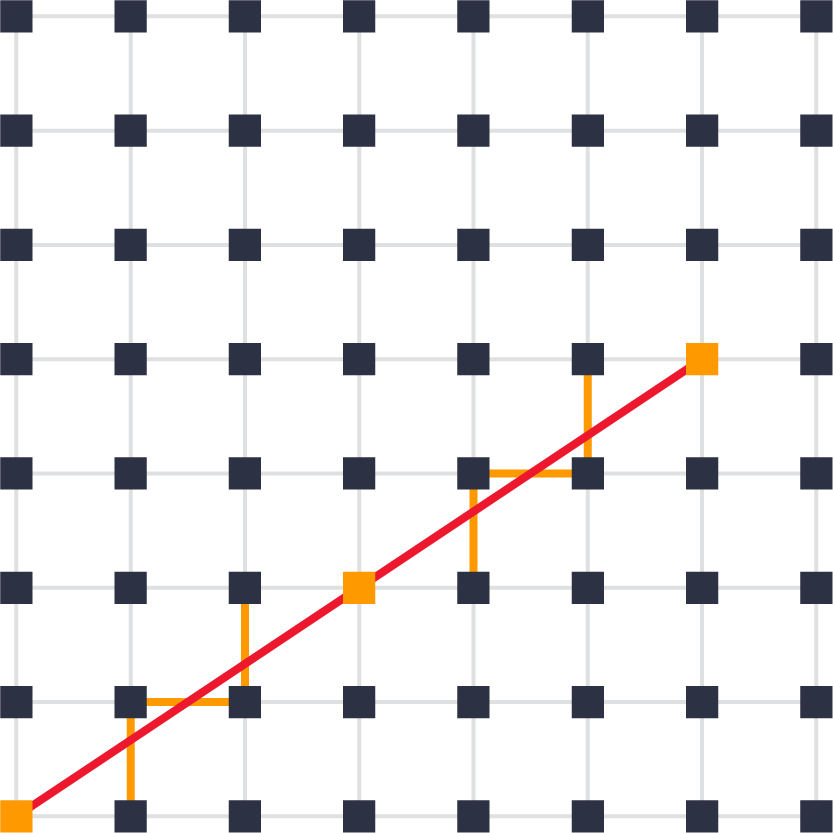
\includegraphics[width=.35\linewidth]{../picture/laser.png}
\end{figure}

위 그림은 $N=7$, $M=7$인 경우 $\left(0, 0\right)$에서 $\left(6, 4\right)$로 레이저를 쏜 모습이다. $3$개의 건물과 $6$개의 벽에 구멍이 뚫린다.

또한, 레이저를 한 번 쏘고 나면 구멍이 뚫린 건물과 벽을 전부 수리할 것이다. 건물을 수리하는 데에는 $A$원, 벽을 수리하는 데에는 $B$원이 든다. 수리를 완료해야 다음 레이저를 쏠 수 있다.

ahgus89의 계획을 들은 Sait2000은 수리비가 얼마나 들 지 생각하며 고민에 빠졌다. Sait2000을 위해 총 수리비를 구해주자!


\InputFile
첫 번째 줄에 $N$, $M$, $A$, $B$가 공백으로 구분되어 주어진다. ($1 \leq N, M, A, B \leq 10^{9}$)

\OutputFile
실험을 완료한 뒤의 총 수리비를 출력한다. 단, 답이 너무 커질 수 있으니 $10^{9}+7$로 나눈 나머지를 출력한다.

\Examples

\begin{example}
\exmp{
1 1 5 6
}{%
40
}%
\exmp{
2 2 3 1
}{%
244
}%
\exmp{
14 15 134 187
}{%
89892000
}%
\end{example}

\Note

\textbf{예제 1}의 상황은 다음과 같다.

$\left(0, 0\right)$에서 $\left(1, 1\right)$로 쏘고 나면 $2$개의 건물을 수리한다.

$\left(1, 0\right)$에서 $\left(0, 1\right)$로 쏘고 나면 $2$개의 건물을 수리한다.

$\left(0, 1\right)$에서 $\left(1, 0\right)$로 쏘고 나면 $2$개의 건물을 수리한다.

$\left(1, 1\right)$에서 $\left(0, 0\right)$로 쏘고 나면 $2$개의 건물을 수리한다.

따라서 총 $8$개의 건물을 수리하므로, 총 수리비는 $40$원이다.

\textbf{예제 2}에서 $\left(0, 0\right)$에서 $\left(2, 2\right)$로 쏘고 나면 $3$개의 건물만을 수리함에 유의하라.

\end{problem}
